\documentclass[11pt]{article}
\ifdefined\pdfinfoomitdate\pdfinfoomitdate=1\fi
\ifdefined\pdfsuppressptexinfo\pdfsuppressptexinfo=-1\fi
\ifdefined\pdftrailerid\pdftrailerid{}\fi
\usepackage[margin=1in]{geometry}
\usepackage{amsmath,amssymb,amsthm}
\usepackage{booktabs,array,graphicx}
\IfFileExists{microtype.sty}{\usepackage{microtype}}{}
\usepackage[hidelinks]{hyperref}
\IfFileExists{result_macros.tex}{\input{result_macros.tex}}{}
\providecommand{\ScienceSnapshot}{\texttt{8a52257fc2829c73d485c7b4c6e310baadfe3c38}}
\newcommand{\dd}{\mathrm{d}}
\newcommand{\Tr}{\operatorname{Tr}}
\newcommand{\spec}{\operatorname{spec}}
\newcommand{\norm}[1]{\left\lVert#1\right\rVert}
\newcommand{\Cov}{\mathsf C}
\newcommand{\Weyl}{\mathcal W}
\newtheorem{proposition}{Proposition}
\hypersetup{pdftitle={Regional Transfer, Geometric Feedback, and Local Memory: A Finite Spherical Realization of Nested-Space Inheritance},pdfauthor={Douglas Ek},pdfsubject={Measured finite spherical realization and conditional local response}}
\title{Regional Transfer, Geometric Feedback, and Local Memory:\\
A Finite Spherical Realization of Nested-Space Inheritance}
\author{Douglas Ek}
\date{1 October 2026}
\begin{document}
\maketitle
\begin{abstract}
We construct a finite spherical realization in which regional state differences,
energy exchange, geometric feedback, maintained localization, and a measurable
local response occur under one action. Six Gaussian fermion columns and the
metric evolve together on a periodic radial chart. A conformal gauge gives
wave transport for the continuum constraints and an explicit forcing budget
for the projected finite dynamics. Four matched runs reach coordinate time
0.3 without a state reset. A localized region remains the leader while
normal energy flows across three natural regional surfaces; the associated
space, time, and quadrature indicators are below one percent. Curvature is
computed from the realized metric and the actual projected time jet, rather
than inferred from an auxiliary field. On the active interval 0.2 to 0.3,
reduction to the original two-mode observer reproduces the generated
occupation and coherence. Memory, initial exterior drive, and actual initial
cross correlations each produce a local effect larger than its independently
measured comparison discrepancy. Source-imbalance controls change transfer and leadership
under the same law. The construction reuses finite normalized inheritance
and standard operator elimination. It demonstrates maintained structure
with regional transport and local memory on a declared finite realization, with
numerical precision indicators; it does not infer a periodic return,
new matter, an eternal continuation, or a continuum state-error certificate.
\end{abstract}

\section{The finite result and its organizing relation}
The question is whether a regional difference can support exchange,
state--geometry feedback, maintained structure, and a local measurement
within the same equations. We exhibit this chain on a finite periodic
spherical chart. The result combines a coupled forward trajectory with
an exact form of reduced dynamics and quantified numerical comparisons.
The spatial window remains populated and carries energy through its
boundaries while the original mode observer changes substantially.

The organizing relation of Nested-Space Cosmology is
\begin{equation}\label{eq:inheritance}
\mathcal T_\Theta^*\mathbb D_\Theta=\mathbb D_\Theta.
\end{equation}
The preserved foundation provides the physical motivation and the
one-spectrum formulation~\cite{EkNSC2026}. Its finite operator companion
specifies normalized inheritance~\cite{EkNested2026}. For a Hermitian
prototype $H$, link $B$, scale $\Omega>0$, and finite depth $N$, the blocks
$(J_{m,N})_{jj}=\Omega^{m+j}H$ and
$(J_{m,N})_{j,j+1}=\Omega^{m+j}B$ obey
\begin{equation}\label{eq:finiteinheritance}
J_{m+1,N}=\Omega U_mJ_{m,N}U_m^\dagger,
\qquad
\spec(\Omega^{-m}J_{m,N})=\spec(J_{0,N}).
\end{equation}
Here $U_m$ relabels corresponding equal-depth windows. Every block gains
one factor $\Omega$, which proves the identity; unitary spectral covariance
then proves the second statement. Standard ordered Schur elimination
preserves the response of the removed blocks.

We reuse this finite distinction between inherited law and regional state.
The present realization fixes one action and source inventory, while
occupations and geometry can differ. Its evolving spatial windows are not
asserted to equal a frozen, hand-selected $H,B$ hierarchy. Geometry changes
the generated Dirac operator and its dressed spectrum. Equation~\eqref{eq:finiteinheritance}
therefore supplies an operator-level construction, not an additional
measured cosmological scaling law.

\section{Declared action, chart, and Gaussian source}\label{sec:model}
We use dimensionless reference units with $\hbar=1$, radial period
$\mathcal L=8$, and the spherical metric
\begin{equation}\label{eq:metric}
\dd s^2=r^2\left[L^2\dd t^2-Q^2(\dd x+\beta\dd t)^2-\dd\Omega_2^2\right].
\end{equation}
The physical lapse and radial metric coefficient are $N=rL$ and $q=rQ$.
The positive chart has $r,Q,L>0$. Spatial geometry is periodic and spinors
are antiperiodic. This is a finite boundary problem, not an asymptotically
flat exterior or a fitted cosmological background.

The selected branch $\Gamma_{\rm one}$ contains the canonical Gaussian
source and a same-spectrum local induced geometric term, counted once.
Spectral-action and heat-kernel methods provide its established
background~\cite{ChamseddineConnes1997,Vassilevich2003}; spherical canonical
reduction is standard~\cite{GrumillerKummerVassilevich2002}. We adopt the
recorded local truncation and coefficients, without claiming a UV completion
or a newly determined set of fundamental constants. After the owned
boundary completion, its first-order geometric density is
\begin{align}\label{eq:lagrangian}
\mathcal L_g={}&2\mathcal K(F_r u+fv)-2F_xL_x/Q
 +Z\left[(Q/L)u^2-(L/Q)r_x^2\right]+LQV,\\
\mathcal K={}&[Q_t-(\beta Q)_x]/L,\quad
u=r_t-\beta r_x,\quad v=\chi_t-\beta\chi_x,\nonumber\\
F={}&-4\pi A r^2+f\chi,\quad f=-8\pi C_W/3,\quad Z=-24\pi A,\nonumber\\
V={}&8\pi A r^2-\frac f2(4\chi+\chi^2)-2\pi C_F b_{\rm mag}^2.\nonumber
\end{align}
Time-cap data are $Q,r,\chi$; the spatial boundary flux integrates to zero.
The Euler and total-divergence terms remain boundary terms on this domain.
The auxiliary $\chi$ linearizes the Weyl term. Its equation supplies
$\chi=R_h-2$ in the continuum action, but the realized metric curvature is
calculated independently in Section~\ref{sec:curvature}.

\begin{table}[tbp]
\centering
\caption{Fixed geometric inputs of the selected local action. Values are
model inputs from the retained same-spectrum record, in reference units.}
\label{tab:inputs}
\begin{tabular}{ll@{\qquad}ll}
\toprule
Coefficient & Value & Coefficient & Value\\
\midrule
$A$ & $0.04501936182826115$ & $C_W$ & $-0.0008441130342798952$\\
$C_F$ & $0.01125484045706527$ & $b_{\rm mag}$ & $4$\\
$C_E$ & $0.0005158468542821582$ & $C_{\Box}$ & $-0.0005627420228532635$\\
$V_{\rm rel}$ & $0$ & $\kappa$ & $1$\\
\bottomrule
\end{tabular}
\end{table}
The nonsingular first-order chart requires $A\ne0$ and $C_W\ne0$.
The magnetic convention is $F_{\theta\phi}=b_{\rm mag}\sin\theta/2$.
The retained input gives $C_Fb_{\rm mag}^2/(4A)=1$; $V_{\rm rel}$ is not
added again to~\eqref{eq:lagrangian}.

The canonical spinor is the half-density $\varphi=r\sqrt q\,\psi$.
One representative angular block has
\begin{equation}\label{eq:dirac}
H(L,Q,\beta)=\sigma_2\frac12\{L/Q,P\}
 +\kappa L\sigma_1-\frac12\{\beta,P\},\qquad P=-i\partial_x.
\end{equation}
Its finite Gaussian covariance is
\begin{equation}\label{eq:covariance}
\Cov=\Phi\,\operatorname{diag}(c)\,\Phi^\dagger,\qquad
c=(0.75,0.75,0.5,0.5,0.25,0.25),\qquad \Phi^\dagger\Phi=I_6.
\end{equation}
Thus $0\le\Cov\le I$ and $\Tr\Cov=3$. Zero occupation of the remaining
band is a finite preparation, not an identification of a physical vacuum.
Gaussian one-body expressions use established fermionic trace
identities~\cite{Klich2003}.

The source consists of three real two-lobe envelopes. With
$b(u)=\exp[-1/(u(1-u))]$ on $0<u<1$ and zero otherwise, the two lobes are
normalized $b(u)$ and $(u-1/2)b(u)$. Packet $n$ combines the even lobe on
$[n,n+1]$ with the odd lobe on $[n+1,n+2]$, followed by real symmetric
orthonormalization. Its plus column has local carrier
$e^{ik(x-n)}f_n(x)(1,i)^T/\sqrt2$, with $k=1$.
The minus column is $e^{i\vartheta}$ times its conjugate,
$\vartheta=-0.842669616901$. This constant column phase does not change
$\Cov$, but the original observer phases are retained for coherence.
The half-density samples include $\sqrt{\Delta x}$.

In this truncation, the state-resolved variational representation is
\begin{equation}\label{eq:combinedaction}
\Gamma_{\rm one}=\int\mathcal L_g\,\dd t\,\dd x+
M\sum_a c_a\int\dd t\,
\left\langle\varphi_a,
\left(\frac{i}{2}\overleftrightarrow{\partial_t}-H\right)
\varphi_a\right\rangle_x .
\end{equation}
The symmetrized time term gives the same canonical field equation and a
real functional. Fixed nonzero weights cancel from that equation, while
remaining in the metric variation. This is the selected local/state branch,
not a second geometric source supplied by the later exterior elimination.
The angular copy weight is $M=4\kappa=4$. It multiplies geometric source
energy and force,
\begin{equation}\label{eq:sourceenergy}
E_f=M\sum_a c_a\langle\Phi_a,H_G\Phi_a\rangle,
\end{equation}
while each representative column evolves by $\dot\Phi_a=-iH_G\Phi_a$.
There is no additional $M$ in this generator or in a modal occupation.

\section{Constraints, conformal formulation, and finite projection}\label{sec:constraints}
The momenta derived from~\eqref{eq:lagrangian} give
$\Pi=p_r-(F_r/f)p_\chi$. Before choosing lapse and shift, their variations
retain the constraints
\begin{align}\label{eq:constraints}
\mathcal C_g={}&\frac{p_Qp_\chi}{2f}+\frac{\Pi^2}{4ZQ}
 +\frac{Zr_x^2}{Q}-QV-2\partial_x(F_x/Q),\\
\mathcal D_g={}&p_rr_x+p_\chi\chi_x-Q\partial_xp_Q.\nonumber
\end{align}
Define the continuum column moments
\begin{align*}
K&=\sum_a c_a\operatorname{Re}(\varphi_a^\dagger\sigma_2P\varphi_a),\\
S_1&=\sum_a c_a\varphi_a^\dagger\sigma_1\varphi_a,\\
J&=\sum_a c_a\operatorname{Re}(\varphi_a^\dagger P\varphi_a).
\end{align*}
The source energy derivatives per coordinate length are
\begin{equation}\label{eq:forces}
\mathfrak f_L=M(K/Q+\kappa S_1),\qquad
\mathfrak f_Q=-MLK/Q^2,\qquad \mathfrak f_\beta=-MJ.
\end{equation}
The total constraints are $\mathcal C=\mathcal C_g+\mathfrak f_L$ and
$\mathcal D=\mathcal D_g+\mathfrak f_\beta$. Source and geometry therefore
belong to the same Hamiltonian variation.

We choose $L=Q$, $\beta=0$ after retaining those constraints. The
Hamiltonian is $H_c=\int h_c\dd x$, with $h_c=Q\mathcal C$.
Differentiation of this $Q$-dependent lapse matters: relative to fixed-lapse
rates evaluated at $L=Q$, the $p_Q$ rate gains $-\mathcal C_g$, and its
matter contribution is $-(\mathfrak f_Q+\mathfrak f_L)$.
This is the chain rule of the gauge-fixed action; it vanishes as an extra
constraint term on the constrained surface. It is not a state correction
or a new radius force. The field generator simplifies to
\begin{equation}\label{eq:conformaldirac}
H_c^{(f)}=\sigma_2P+\kappa Q\sigma_1.
\end{equation}
The kinetic coefficient is one; geometry remains in the angular mass
term and in the physical metric.

\begin{proposition}[Continuum constraint transport]\label{prop:transport}
For smooth periodic fields in the positive chart, the Hamiltonian
$\int Q\mathcal C\dd x$ derived above satisfies
\begin{equation}\label{eq:constraintwaves}
\partial_t h_c=\partial_x\mathcal D,\qquad
\partial_t\mathcal D=\partial_xh_c.
\end{equation}
\end{proposition}
\begin{proof}
Set $a=F_{rr}=-8\pi A$, so $F_r=ar$ and $Z=3a$.
Differentiate~\eqref{eq:constraints} with the canonical equations in
Appendix~\ref{app:rates}. The spatial derivatives in $F_x/Q$ supply the
improved momentum density $-Qp_{Q,x}$. The field equations
$ i\varphi_t=(\sigma_2P+\kappa Q\sigma_1)\varphi$ give the derivatives of
$K,S_1,J$ in~\eqref{eq:forces}. Their angular-mass terms cancel the
$-M\kappa S_1$ term in $\dot p_Q$. The remaining terms are respectively
$\partial_x\mathcal D$ and $\partial_x(Q\mathcal C)$.
This calculation uses $V_r=-2ar$ and $V_\chi=-f(2+\chi)$; the constant
magnetic term differentiates to zero. It applies column by column and
therefore to arbitrary fixed Gaussian weights. Independent symbolic
Euler derivatives and directional checks reproduce the identities.
\end{proof}
Consequently vanishing smooth constraints propagate homogeneously.
The numerical projection is kept distinct from this continuum identity.

Geometry uses the odd periodic band $n_g=n_f-1$ and the columns use the
even antiperiodic band $n_f$. Both are prolonged to $n_q=4n_f$ quadrature
nodes. With $A_g,A_f$ the nodal interpolation maps,
\begin{equation}\label{eq:maps}
P_g=\frac{n_g}{n_q}A_g^T,\qquad
U_f=\sqrt{n_f/n_q}\,A_f,\qquad
P_gA_g=I,\quad U_f^\dagger U_f=I.
\end{equation}
The fine Hamiltonian is evaluated on the prolonged state, and every
geometric and field rate is pulled back by the exact respective adjoint.
In particular $H_G=U_f^\dagger H_c^{(f)}U_f$ is Hermitian.
Products use the summation-by-parts energy and the actual discrete
$\mathsf D_xF$, not a silently imposed continuum product rule.

For the actual finite ODE, define the full quadrature defects
\begin{equation}\label{eq:forcing}
f_h=\dot h_c-\mathsf D_x\mathcal D,\qquad
f_D=\dot{\mathcal D}-\mathsf D_xh_c,\qquad
R^2=\Delta x_q\sum(h_c^2+\mathcal D^2).
\end{equation}
Skew adjointness of $\mathsf D_x$ yields
\begin{equation}\label{eq:budget}
\frac{\dd R^2}{\dd t}=2\Delta x_q\sum(h_cf_h+\mathcal D f_D),\qquad
R(t)\le R(0)+\int_0^t\norm{(f_h,f_D)}_2\dd s.
\end{equation}
Analytic directional derivatives of the actual sampled constraints expose
both unprojected quadrature forcing and the additional rate-projection
forcing. Neither is discarded. Equation~\eqref{eq:budget} is a finite ODE
estimate without an exponential in the Fourier cutoff. Its sampled time
integral is a numerical indicator, not a certified continuum enclosure.

\section{Forward episodes and maintained regional transfer}\label{sec:episodes}
The initial $Q=0.251324933269135$ is constant; $\chi$ and the momenta start
at zero in the retained baseline. The radius is the saved source-derived
solution of the projected lapse constraint. Initial source and intrinsic
and extrinsic data do not change when choosing the conformal gauge,
because $\mathfrak f_L,\mathfrak f_\beta$ are independent of $L,\beta$.
The near-zero initial current is reported rather than subtracted.

Four runs use $n_f=256,512$ and step caps $0.001,0.0005$.
The first episode reaches $T=0.05$; the second continues each corresponding
Cauchy state bitwise to $T=0.3$. Each RK4 stage recomputes the source,
geometric rates, and Dirac image on that stage state. The next step is
bounded by $1.4/\omega$, where
$\omega=k_{\max}+\kappa\max Q$, and by the output-frame endpoint.
All four runs remain in the positive chart with column Gram errors below
$5.3\times10^{-12}$; the fine half-step case stays below
$1.7\times10^{-13}$ during the continuation.

\begin{table}[tbp]
\centering
\caption{Initial and final full constraint diagnostics. These are sampled
norms, separately reported from projected solver residuals.}
\label{tab:constraints}
\begin{tabular}{lrrrr}
\toprule
$n_f$, step cap & $\norm{\mathcal C(0)}_\infty$ & $R(0)$ & $R(0.3)$ & $R_{\rm budget}(0.3)$\\
\midrule
256, $0.0005$ & $1.7681\!\times\!10^{-3}$ & $2.9599\!\times\!10^{-4}$ & $2.9761\!\times\!10^{-4}$ & $3.9497\!\times\!10^{-4}$\\
512, $0.0005$ & $9.9815\!\times\!10^{-6}$ & $2.0955\!\times\!10^{-6}$ & $2.0862\!\times\!10^{-6}$ & $4.3987\!\times\!10^{-4}$\\
\bottomrule
\end{tabular}
\end{table}
Table~\ref{tab:constraints} states the initial residual domain explicitly.
The fine endpoint has full maxima $\norm{\mathcal C}_\infty\simeq
9.00\times10^{-6}$ and $\norm{\mathcal D}_\infty\simeq7.98\times10^{-7}$.
The forcing integral is not asserted to decrease with resolution: its fine
joined value is about $4.38\times10^{-4}$, dominated by rate projection.
This constraint-control primitive and the physical refinement indicators
answer different questions; the initial full residual is part of the
declared numerical domain.

The four natural spatial windows are $I_j=[2j,2j+2]$, $j=0,\ldots,3$.
Contents are exact integrals of the periodic nodal trigonometric
interpolants on those intervals. Let $V_x=4\pi r^2q$ be physical volume
per coordinate length. The normal-observer shell and canonical probability
are
\begin{equation}\label{eq:contents}
E_N(I)=\int_I V_x\rho_N\dd x,\qquad
\mathcal P(I)=\sum_a c_a\int_I\varphi_a^\dagger\varphi_a\dd x.
\end{equation}
The normal shell is the nodal sum of $F_L/r$. This differs from the
coordinate Hamiltonian energy and from a two-mode occupation.

\begin{figure}[tbp]
\centering
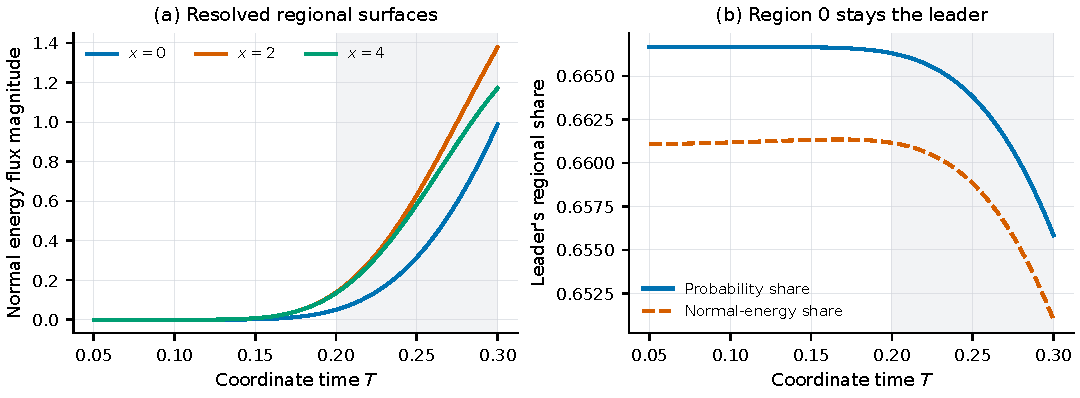
\includegraphics[width=.95\linewidth,height=.27\textheight,keepaspectratio]{figures/regional-transfer.pdf}
\caption{Continuation of the same realization on $0.05\le T\le0.3$:
individual physical surface flows and the region-0 shell and probability
shares. The handoff at $0.05$ continues the full Cauchy state of the first
episode. Energy flow is separated from canonical probability and from the
fixed mode-observer measurement.}
\label{fig:transfer}
\end{figure}

Region 0 remains the normal-shell and probability leader throughout.
During the continuation its shares stay above $0.65098$ and $0.65585$.
Its normal shell changes from $6.62107371$ at $0.05$ to $6.57976032$ at
$0.3$; its probability content falls by $0.03246364$.
Maintenance here means persistence of the localized leader during regional
transport. Its shell and probability contents decrease; the individual
leader-surface flows can both point outward. Equal entry and exit, constant
content, circulation, and recovery of an identical state are not inferred.
The finite interval was extended because outer-boundary
flow at $0.05$ was unresolved, despite resolved internal current.

For outward normal-energy flux $\mathcal J_N$, each surface is assessed
individually through $\int|\mathcal J_N|\dd t$ as well as its signed
integral. Opposing nonzero entry and exit can cancel in a net-content
balance and are not rejected for that reason.
\begin{table}[tbp]
\centering
\caption{Absolute normal-energy-flow integrals during $T\in[0.05,0.3]$.
Indicators are movement divided by each surface's own flow effect.}
\label{tab:flow}
\begin{tabular}{lrrrr}
\toprule
Surface & Integral & time indicator & space indicator & frame quadrature\\
\midrule
$x=0$ & $0.03937795$ & $4.41\times10^{-7}\%$ & $0.00214\%$ & $0.09503\%$\\
$x=2$ & $0.07025487$ & $5.81\times10^{-7}\%$ & $0.00636\%$ & $0.04273\%$\\
$x=4$ & $0.06351828$ & $6.17\times10^{-7}\%$ & $0.00134\%$ & $0.03139\%$\\
\bottomrule
\end{tabular}
\end{table}
The fourth distinct surface, $x=6$, is unresolved on this realization.
The three reported exchanges satisfy the declared one-percent numerical
criterion in their stated windows; that label is not applied to every
constraint diagnostic or to a total continuum error.

\subsection{Coordinate work and the normal shell ledger}\label{sec:ledger}
The geometry exchanges energy with the field through the same variation.
If $F_i$ are nodal energy derivatives, coordinate work is
\begin{equation}\label{eq:coordinatework}
\dot E_f=\sum(F_Q\dot Q+F_L\dot L+F_\beta\dot\beta)
=\sum(F_Q+F_L)\dot Q_{\rm lifted}.
\end{equation}
There is no extra spacing or angular multiplicity in this nodal sum.
Using only $F_Q\dot Q$ would omit the evolving lapse. Across both fine
episodes the field-energy change is about $-2.37443\times10^{-5}$,
balanced by the geometric change to $1.31\times10^{-11}$.

For the normal observer, define expansion rates
$K_r=[q_t-(\beta q)_x]/(Nq)$ and
$K_\perp=(r_t-\beta r_x)/(Nr)$. The continuum shell balance is
\begin{align}\label{eq:normalbalance}
\partial_t(V_x\rho_N)+\partial_x\mathcal J_N&=\mathcal W_p+\mathcal W_N,\\
\mathcal J_N&=V_x(Nj_N/q-\beta\rho_N),\nonumber\\
\mathcal W_p&=-NV_x(p_r^{(N)}K_r+2p_\perp^{(N)}K_\perp),\nonumber\\
\mathcal W_N&=-V_x(j_N/q)N_x.\nonumber
\end{align}
The source derivatives give the stresses, for example
$\rho_N=\mathfrak f_L/(4\pi r^4Q)$ and
$j_N=-\mathfrak f_\beta/(4\pi r^4Q^2)$.
The realized finite balance includes its measured directional residual,
which is retained rather than zeroed.
For region 0 on $[0.05,0.3]$, frame-Simpson integrals of net boundary
flow, pressure work, and lapse-gradient work are approximately
$-0.10956538$, $+0.04884147$, and $+0.01941054$.
They account for the shell change $-0.04131339$ to about
$1.99\times10^{-8}$; the trapezoid balance indicator is about $0.164\%$
of that shell change.

\begin{figure}[tbp]
\centering
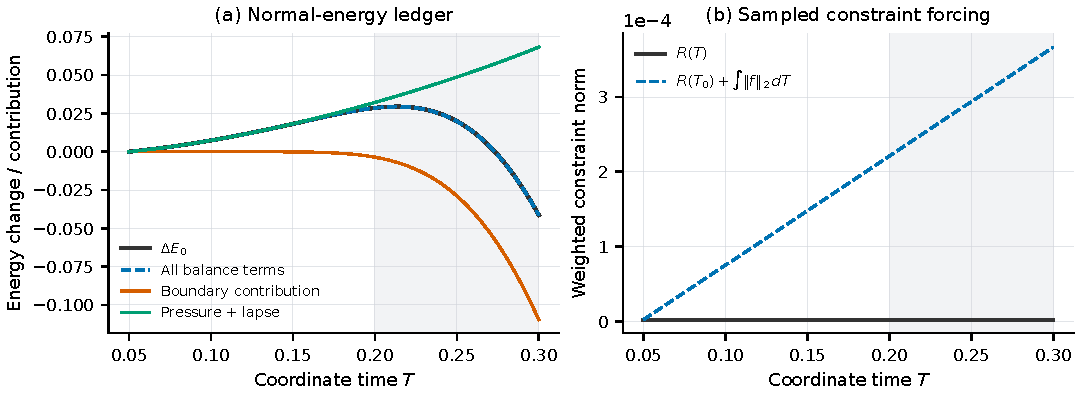
\includegraphics[width=.95\linewidth,height=.25\textheight,keepaspectratio]{figures/normal-ledger.pdf}
\caption{Normal-observer shell accounting (left): boundary flow, pressure
work and lapse-gradient work are distinct from coordinate field--geometry
energy exchange. The sampled constraint norm and integrated forcing budget
(right) use~\eqref{eq:budget}; the sampled integral is not a certified
continuum or temporal bound.}
\label{fig:ledger}
\end{figure}

\section{Realized curvature and the proper-clock control}\label{sec:curvature}
The metric itself supplies an invariant measurement. In the conformal
chart, $\dot Q_g=P_g[Q_fp_{\chi,f}/(2f)]$.
Differentiating this actual finite rate along the actual projected ODE gives
\begin{equation}\label{eq:qjet}
\ddot Q_f=A_gP_g\left[
\frac{\dot Q_f p_{\chi,f}+Q_f\dot p_{\chi,f}}{2f}\right],\qquad
\dot Q_f=A_g\dot Q_g,\quad \dot p_{\chi,f}=A_g\dot p_{\chi,g}.
\end{equation}
Both projections and $\dot L=\dot Q_f$ are kept.
The two-metric scalar and spherical Weyl invariant are
\begin{equation}\label{eq:curvature}
R_h=\frac{2}{Q^2}\left[\frac{Q_{xx}}Q-\frac{Q_x^2}{Q^2}
-\frac{\ddot Q}Q+\frac{\dot Q^2}{Q^2}\right],\qquad
\Weyl=C_{\mu\nu\rho\sigma}C^{\mu\nu\rho\sigma}
=\frac{(R_h-2)^2}{3r^4}.
\end{equation}
The second identity is the owned conformal spherical product relation.
Directional differences of the finite rate validate~\eqref{eq:qjet}; an
independent Christoffel contraction validates the metric sign and factors.

At the fine $T=0.3$ endpoint,
$R_h\in[11.45342664,15.71659763]$ and
$\max\Weyl=0.11331608321$.
Its spatial indicator is $0.00110\%$, and its timestep movement is about
$5.13\times10^{-11}$.
Only after this calculation is the auxiliary relation compared:
$\max|R_h-(\chi+2)|\simeq7.88\times10^{-8}$ and the maximum pointwise
Weyl/proxy gap is about $1.29\times10^{-9}$.
The dense and FFT realizations of the same spatial derivative differ in
finite precision, with a recorded endpoint curvature-formula gap
$2.64\times10^{-6}$. This conditioning indicator is distinguished from
an exact-arithmetic identity or a continuum enclosure.

\begin{figure}[tbp]
\centering
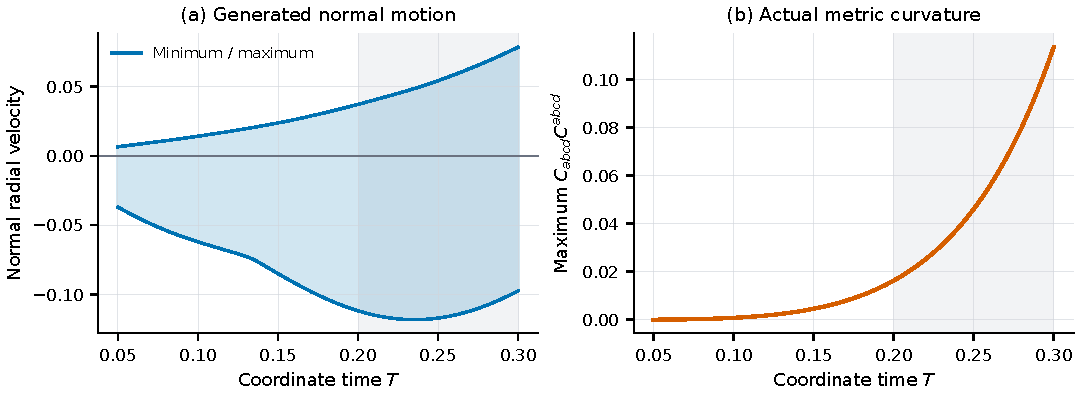
\includegraphics[width=.95\linewidth,height=.27\textheight,keepaspectratio]{figures/geometry-curvature.pdf}
\caption{Normal radial motion and actual metric curvature on the generated
positive chart. The Weyl invariant is computed from the projected ODE time
jet and spatial metric jet; agreement with the auxiliary proxy is assessed
afterward. The endpoint proper-clock control uses this same metric.}
\label{fig:geometry}
\end{figure}

The reference normal worldline is fixed at $x=1$, with
$\dd\tau=rQ\dd t$. Its clock is continuous from $T=0$ and reaches
$\tau=0.3616114057$ at $T=0.3$.
The frozen-geometry control keeps the original $Q_0$ and columns. Its
constant generator has modal frequencies
$\sqrt{p^2+\kappa^2Q_0^2}$, so its propagation is evaluated analytically.
At the same normal-clock endpoint, the original observer's two occupation
separations are approximately
$(-1.19109,-1.06846)\times10^{-5}$.
Their time and space indicators are below $0.0008\%$ and $0.00014\%$.
No interpolation of the frozen control or reset of the clock is required.
Most occupation change is also present in frozen geometry; this smaller
resolved separation identifies the measured geometric contribution under
the declared observer and clock protocol.

\section{Source-imbalance controls under the same law}\label{sec:sourcecontrols}
The source family
\begin{equation}\label{eq:alphasource}
c(\alpha)=(\tfrac12+\tfrac14\alpha,\tfrac12+\tfrac14\alpha,
\tfrac12,\tfrac12,\tfrac12-\tfrac14\alpha,\tfrac12-\tfrac14\alpha)
\end{equation}
preserves total occupation three and equal weights inside each conjugate
pair. Four exploratory coarse runs use $\alpha=0,-1,0.95,1.05$.
The original columns are unchanged; the source radius and periodic shift
momentum are solved anew at the initial slice, and the current mean remains
in the shift residual. Full initial Hamilton maxima range from
$0.00137$ to $0.00179$ and retain their declared solver-floor domain.
All four runs reach $0.3$, keep a positive chart and Gram gaps below
$1.7\times10^{-13}$, and have positive sampled forcing-budget margins.

Reversal changes the signed transfer at $x=2$ from about $+0.07025$ to
$-0.07024$ and moves the maintained normal-shell leader to region 1.
The $\pm5\%$ imbalance perturbations keep region 0 as leader and change
that transfer by approximately $\pm5.04\%$. The changes at $x=4$ are
approximately $\mp4.86\%$. Paired frame-quadrature indicators are about
$0.043\%$ and $0.031\%$ of those measured differences.
These coarse controls establish source sensitivity; the baseline's fine
comparisons are reference scales, not a control-specific continuum error
certificate.

Uniform weights leave substantial outer flow: about $0.02664$ at $x=0$
and $0.12415$ at $x=4$. They represent half of a rank-six projector,
not half the identity on the full band. The empty complement remains
available to the dynamics. The uniform run has two comparably occupied
windows and changes its normal-shell leader; no minimum-share or reversal
condition is imposed to hide that outcome.

\section{The same realization seen by a fixed mode observer}\label{sec:local}
A spatial energy window and a Hilbert-space observer are distinct.
Let $V$ be the original $T=0$ columns 0 and 1, preserved without QR,
phase change or transport to a new observer. Its projector is $P_A=VV^\dagger$.
The complement $P_E=I-P_A$ includes modes with support inside and outside
$[0,2]$. Throughout, $E$ means exterior to the retained \emph{mode space}.
The omission controls do not isolate a contribution solely from a geometric
parent region or attribute the response to only the $x=2$ surface.
The local measurements are the two diagonal occupations and the
complex off-diagonal coherence of $V^\dagger\Cov V$.
They are not identified with integrated shell energy or with the window's
canonical probability.

The reduction starts with the actual transported $\Phi(0.2)$,
not the original columns placed again at the segment boundary.
At that point the local covariance eigenvalues are approximately
$0.103233,0.107916$, and the actual initial cross norm is
$\norm{C_{AE}}_F=0.3386366$.
The original weights remain those in~\eqref{eq:covariance}.
Generated $Q$ is prolonged to the original quadrature and linearly
interpolated between the 21 stored frames on $[0.2,0.3]$.
This defines the conditional field schedule used by both full and reduced
propagation. Independent Fourier actions match the generated Galerkin
operator to below $4.4\times10^{-13}$ relative error.

\subsection{Exact elimination and actual initial correlations}
In the fixed orthonormal frame $[V,V_E]$, write
$H_G(t)=\left(\begin{smallmatrix}A&B\\B^\dagger&D_E\end{smallmatrix}\right)$.
The free exterior propagator obeys
$i\partial_tU_E(t,s)=D_E(t)U_E(t,s)$ and $U_E(s,s)=I$.
For retained and exterior column amplitudes $x,y$, integration of the
exterior equation gives
\begin{align}\label{eq:elimination}
y(t)&=U_E(t,t_*)y_* -i\int_{t_*}^tU_E(t,s)B^\dagger(s)x(s)\dd s,\\
\dot x(t)&=-iA(t)x(t)-iB(t)U_E(t,t_*)y_*
 -\int_{t_*}^tK(t,s)x(s)\dd s,\nonumber\\
K(t,s)&=B(t)U_E(t,s)B^\dagger(s),\qquad t_*=0.2.\nonumber
\end{align}
Thus unresolved degrees remain as causal memory and initial exterior
drive. The initial covariance contributes cross terms as well as its two
marginals. For the exact responses $R_A,R_E$ from each initial component,
\begin{align}\label{eq:localcov}
C_A(t)={}&R_AC_{AA}R_A^\dagger+R_EC_{EE}R_E^\dagger\nonumber\\
 &+R_AC_{AE}R_E^\dagger+R_EC_{EA}R_A^\dagger.
\end{align}
This follows directly by expanding the covariance of the summed amplitude.
It is standard block elimination, applied here to the generated metric and
actual correlated state, rather than a new quantum law.

The streamed solver transports twelve columns: the retained and exterior
pieces of each of the six actual columns. Linearity permits their coherent
sum to reconstruct the original state. Summing the two component
covariances instead removes only the actual initial cross.
Retaining only the first component supplies the initial-drive omission.
An unsplit pilot and independent full split verify these identities.
Time-indexed dense exterior propagators are unnecessary; the stored
column history has shape $(21,1022,12)$.

\subsection{Measured response and individually verified controls}
The two autonomous occupations have the endpoints
\begin{align*}
\boldsymbol n(0.2)&=(0.1055744772,0.1055746375),\\
\boldsymbol n(0.3)&=(0.0321449576,0.0322689986).
\end{align*}
The maximum occupation and coherence changes are $0.0734295196$ and
$0.00237420793$, respectively.

The streamed/full occupation discrepancy is $6.3508\times10^{-6}$,
or $0.00865\%$ of its effect; the coherence discrepancy is
$8.4787\times10^{-7}$, or $0.03571\%$.
The conditional full occupation differs from the saved autonomous frames
by only $2.2951\times10^{-10}$.

\begin{table}[tbp]
\centering
\caption{Causal omissions on the same generated geometry, with each
control's own independent reference error. These are conditional controls,
not separate coupled geometric evolutions.}
\label{tab:localcontrols}
\begin{tabular}{lrrr}
\toprule
Omission & Occupation movement & Own reference error & Error/effect\\
\midrule
Memory & $0.0168185383$ & $2.2011\times10^{-6}$ & $0.01309\%$\\
Initial exterior drive & $0.0485412050$ & $1.6626\times10^{-5}$ & $0.03425\%$\\
Actual initial cross & $0.0920614328$ & $1.2282\times10^{-5}$ & $0.01334\%$\\
\bottomrule
\end{tabular}
\end{table}
Memory omission is independently compared with the triangular generator
$G=H_G-P_EH_GP_A$, which prevents retained-to-exterior feedback while
preserving the retained rows. It is explicitly a non-Hermitian negative
control, not a replacement physical model. Its two-to-four midpoint-substep
indicator is $3.15\times10^{-11}$.
The drive omission is compared with full propagation from the actual
retained initial component. The cross omission is compared with the full
propagation of both actual components, with their cross removed only in
covariance assembly. No synthetic initial cross is inserted.

Doubling full midpoint substeps and replacing linear $Q$ interpolation
with rate-Hermite interpolation using the actual stored $\dot Q=\dot L$
move occupation and coherence by less than one percent of their respective
effects. Geometry-only comparisons retain the primary state and observer
while substituting the time- or space-refined $Q$ path on a common
quadrature. Separately, the actual autonomous occupation differs by
$1.33\times10^{-8}$ across spatial refinement and
$2.32\times10^{-11}$ across timestep refinement.
These declared-path comparisons do not enclose an unknown unstored metric.

\begin{figure}[tbp]
\centering
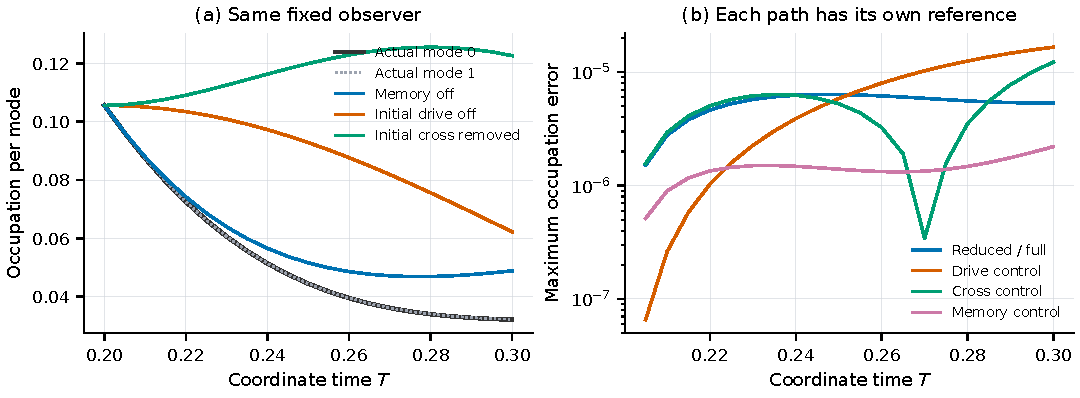
\includegraphics[width=.95\linewidth,height=.27\textheight,keepaspectratio]{figures/local-response.pdf}
\caption{The original fixed observer's autonomous occupations (modes 0 and
1) and mode-0 omission curves on $T\in[0.2,0.3]$ (left), using the actual
$\Phi(0.2)$ correlations. The modal complement is distinct from the spatial
windows. Reduced/full and independent-control comparison errors are maxima
over the two modes (right), using Table~\ref{tab:localcontrols}. The initial
roundoff sample is omitted from the error panel; coherence is independently
quantified in the text.}
\label{fig:local}
\end{figure}

On the same active segment, the three surface values are ordered as
$x=0,2,4$. Their absolute normal-energy-flow integrals, largest numerical
indicators, and the continuous normal-clock endpoints are
\begin{align*}
\text{surface integrals}&=(0.03848436,0.06757848,0.06088737),\\
\text{largest indicators}&=(0.08449\%,0.02699\%,0.01429\%),\\
(\tau(0.2),\tau(0.3))&=(0.2412093356,0.3616114057).
\end{align*}
The spatial leader persists while the fixed observer loses
occupation, and the unresolved complement actively changes that response.
This is the quantitative outside-to-local meaning supported by the
calculated memory and initial-state terms.

\section{Interpretation, limits, and reproducibility}\label{sec:scope}
The established chain is finite: a declared regional Gaussian difference
produces transfer; the same action evolves both state and geometry;
a localized leader persists with resolved boundary flow; and its generated
metric and correlated state support an accurately reproduced local response.
The source controls demonstrate sensitivity under the same law, while the
frozen-clock comparison isolates a smaller geometric contribution.
No periodically renewed state, new matter inventory, or eternal continuation
is inferred. ``Regeneration'' here denotes maintained structure with
regional transport over the measured interval.

Analytic and numerical statements are separate. Normalized finite
inheritance, Hamiltonian variation, block elimination, and the finite ODE
energy identity are algebraic results in stated domains. The trajectory,
surface-flow and local-response values are observations with spatial,
temporal and quadrature indicators. The latter satisfy the declared
one-percent criterion for the reported effects, but are not a total state
error certificate against an unknown geometry or a continuum solution.
In particular, sampled constraint forcing does not by itself provide the
missing physical-observable stability map.
A conditional Duhamel estimate illustrates the additional quantity needed:
if $e$ is a weighted column-state error under a controlled Hamiltonian
mismatch, then
\begin{equation}\label{eq:duhamel}
e(t)\le e(t_*)+\int_{t_*}^t\norm{\delta H(s)\Phi(s)c^{1/2}}_F\dd s,\qquad
\norm{\delta C_A(t)}_F\le2a(t)e(t)+e(t)^2,
\end{equation}
where $a$ is the reference weighted-column norm. The unknown geometric
mismatch is not bounded by the present measurements.
The local memory result also does not identify its Hilbert-space complement
with a new dark stress, antimatter sector, or cosmological abundance.

The machine-readable evidence consists of the versioned JSON/NPZ records
in Table~\ref{tab:evidence}, under \texttt{lab/results/development}.
Input, code and payload hashes are bound in the records and the accompanying
publication manifest. It pins the scientific snapshot
\begin{center}\ScienceSnapshot\end{center}
The preserved source history distinguishes measured
producers from later write-protection wrappers. No sealed trajectory is
silently regenerated for the article.

\begin{table}[tbp]
\centering
\caption{Machine-readable scientific evidence. Basenames are followed by
the listed version and a JSON or NPZ extension as applicable.}
\label{tab:evidence}
\begin{tabular}{lll}
\toprule
Component & Record basename & Versions\\
\midrule
Episodes & \texttt{nsc-spherical-conformal-episode} & v1, v2\\
Physical frames & \texttt{nsc-spherical-conformal-frames} & v1\\
Surface transfer & \texttt{nsc-spherical-conformal-transport} & v2\\
Proper clock & \texttt{nsc-spherical-conformal-clock} & v2\\
Source controls & \texttt{nsc-spherical-conformal-source-controls} & v1\\
Metric invariant & \texttt{nsc-spherical-conformal-curvature} & v1\\
Local response & \texttt{nsc-conformal-local-response} & v2\\
Memory reference & \texttt{nsc-conformal-memory-control} & v1\\
\bottomrule
\end{tabular}
\end{table}

The first episode and its physical postprocessing used about 127 CPU
seconds; continuation used 114 and 493 seconds in its coarse and fine pools.
The four exploratory source controls used 388 seconds, metric curvature
13 seconds, and local production with its independent controls 84 seconds.
The independent memory reference used another 3.64 seconds.
These bounded computations forecast cost before expansion and preserve
full Cauchy handoffs or compact source-control checkpoints.
For read-only local verification, run
\begin{quote}\small\ttfamily
python scripts/lab.py \textbackslash\\
scripts/derive\_nsc\_conformal\_local\_response\_successor.py --check
\end{quote}
Scientific tests separately replay operator actions, directional derivatives,
source bindings, control identities and saved numerical indicators.
The build manifest binds this source, bibliography, figures, evidence and
PDF. The broad foundational manuscript and earlier focused source remain
historical documents of the same programme.

\section*{Author responsibility and assistance}
Substantial AI assistance was used in derivations, implementation, numerical
verification, independent checks, and manuscript preparation. Douglas Ek
is the sole author and is responsible for the scientific claims, evidence
selection, and final manuscript.

\appendix
\section{Continuum equations of the conformal Hamiltonian}\label{app:rates}
For $a=-8\pi A$, $F_r=ar$, $Z=3a$, and
$\Pi=p_r-ar p_\chi/f$, the geometric velocities are
\begin{align}
\dot Q&=Qp_\chi/(2f),&
\dot r&=\Pi/(2Z),&
\dot\chi&=Qp_Q/(2f)-(ar/f)\Pi/(2Z).
\end{align}
The momentum equations, including the same matter source, are
\begin{align}
\dot p_Q&=-p_Qp_\chi/(2f)+2QV+2F_{xx}/Q-M\kappa S_1,\\
\dot p_r&=\Pi a p_\chi/(2Zf)+2Zr_{xx}+Q^2V_r
 +ar\partial_x(2Q_x/Q),\\
\dot p_\chi&=Q^2V_\chi+f\partial_x(2Q_x/Q),
\end{align}
with $i\varphi_t=(\sigma_2P+\kappa Q\sigma_1)\varphi$.
For a single column $\varphi=(u+iv,w+iz)^T$, this field equation reads
$\dot u=-z_x+\kappa Qz$, $\dot v=w_x-\kappa Qw$,
$\dot w=v_x+\kappa Qv$, $\dot z=-u_x-\kappa Qu$.
It gives the bilinears
$K=-uw_x-vz_x+wu_x+zv_x$,
$S_1=2(uw+vz)$ and
$J=uv_x-vu_x+wz_x-zw_x$, weighted and summed over columns.
Substitution gives Proposition~\ref{prop:transport}.
The displayed $2F_{xx}/Q$ is a continuum product-rule simplification;
the finite implementation differentiates its summation-by-parts energy
and retains $\mathsf D_xF$ and the sampled constraint term before pullback.

\bibliographystyle{unsrt}
\bibliography{references}
\end{document}
